\section{Introduction}

Large language models (LLMs) have achieved remarkable progress across diverse tasks, yet they remain prone to generating inconsistent or incorrect outputs, particularly in open-ended or reasoning-intensive scenarios~\citep{wang2022self, huang2025survey}. A common strategy to improve reliability is best-of-$N$ sampling: generate multiple candidate responses from the same prompt and select the highest-quality one according to a scoring mechanism~\citep{cobbe2021training, wang-etal-2024-math, kang2025scalable}. In this framework, performance critically depends not only on the diversity of sampled candidates but, more importantly, on the effectiveness of the selection criterion.

Existing selection methods can be broadly categorized into two groups. The first relies on \emph{external evaluators}, such as reward models or verifiers, to score each candidate~\citep{cobbe2021training, lightman2023let}. While effective, these approaches introduce additional computational overhead and require extra supervision. The second group uses \emph{intrinsic signals} derived from the sampled responses themselves. The dominant paradigm in this category is self-consistency via majority voting, which assumes that correct answers appear most frequently among samples~\citep{wang2022self}. This works well when the answer space is discrete, but it struggles in settings with semantic ambiguity or when high-quality minority answers are underrepresented despite being semantically close to the consensus~\citep{chen2023universal, kang2025scalable}.
Recent work has also proposed ranked or reasoning-aware extensions of self-consistency, such as Borda-style voting, along with theoretical analyses connecting Best-of-$N$ to mode estimation and KL-constrained optimization~\citep{gui2024bonbon, wang2025ranked, wan2025reasoning, cordero2025certified}. Parallel efforts explore weighted aggregation and hybrid selection strategies, such as correlation-aware multi-agent weighting and Best-of-Majority, to improve reliability and scaling behavior~\citep{ai2025beyond, di2025best}.

However, these approaches often rely on additional sampling or surface-form agreement, limiting their practicality in real-world settings, especially when efficient, black-box-compatible, and training-free selection is required. 
As illustrated in Figure~\ref{fig:overview}, these limitations arise from a mismatch between surface-level signals and the underlying semantic structure of candidate answers.
This raises a central question: \emph{Can we develop an efficient and training-free selection framework that operates directly in answer space, enabling robust per-sample ranking without relying on external supervision or costly sampling procedures?}
% ============

To tackle this question, we introduce the \textbf{Radial Consensus Score (RCS)}, a principled geometric approach for efficient best-of-N selection. Our key insight is to model semantic consensus explicitly via a weighted Fréchet mean~\citep{fletcher} as the semantic center of answer embeddings and then rank candidates by their radial distance to this center. This formulation naturally incorporates both semantic agreement structure and optional confidence signals (frequency, generation probability, or pairwise cosine similarity) through the choice of weighting distribution $P$.
Different choices of $P$ recover a spectrum of selection strategies, ranging from uniform weighting that treats all candidates equally to frequency-based, probability-based, and cosine-similarity-based schemes that emphasize consensus, model confidence, or mutual agreement. This flexibility allows the framework to adapt to different inference settings while remaining fully training-free and black-box compatible.
The resulting score is computationally lightweight, model-agnostic, and directly yields a ranking of individual candidates without requiring clustering or external verifiers.
We evaluate RCS on seven established benchmarks spanning short-form QA (SciQ, GPQA), mathematical reasoning (Arithmetics, GSM8K), and long-form multiple-choice tasks (MMLU Formal Logic, MMLU-Pro, BigBenchHard), using five diverse open-weight models. RCS variants consistently outperform strong baselines---including Semantic Consensus Weighting (SCW)---by 2--7\% in selection accuracy, with gains becoming more pronounced as the sampling budget increases. Additional analyses confirm their efficiency and robustness in black-box settings and multi-agent debate scenarios.
Our contributions are threefold:
\textbf{First}, we introduce Radial Consensus Score (RCS), a geometric consensus framework for best-of-$N$ selection that bridges probability-based and surface-form methods, and prove, under a Gaussian generative model, that it outperforms voting in both infinite- and finite-sample regimes under sufficient semantic-separation conditions.
% \textbf{First}, we introduce Radial Consensus Score (RCS), a geometric consensus framework for best-of-$N$ selection that bridges probability-based and surface-form methods, grounded in a closed-form formulation via the Fréchet mean and its discrete medoid counterpart. 
\textbf{Second}, comprehensive experiments across diverse tasks and models demonstrate that RCS consistently outperforms strong baselines, with gains increasing as the sampling budget grows, highlighting favorable scaling behavior.
\textbf{Third}, ablation studies further confirm the effectiveness and applicability of RCS, showing its robustness in multi-agent debate and fully black-box settings, along with strong practical efficiency, underscoring its impact as a scalable aggregation method for LLM inference.


\begin{figure*}[t]
    \centering
    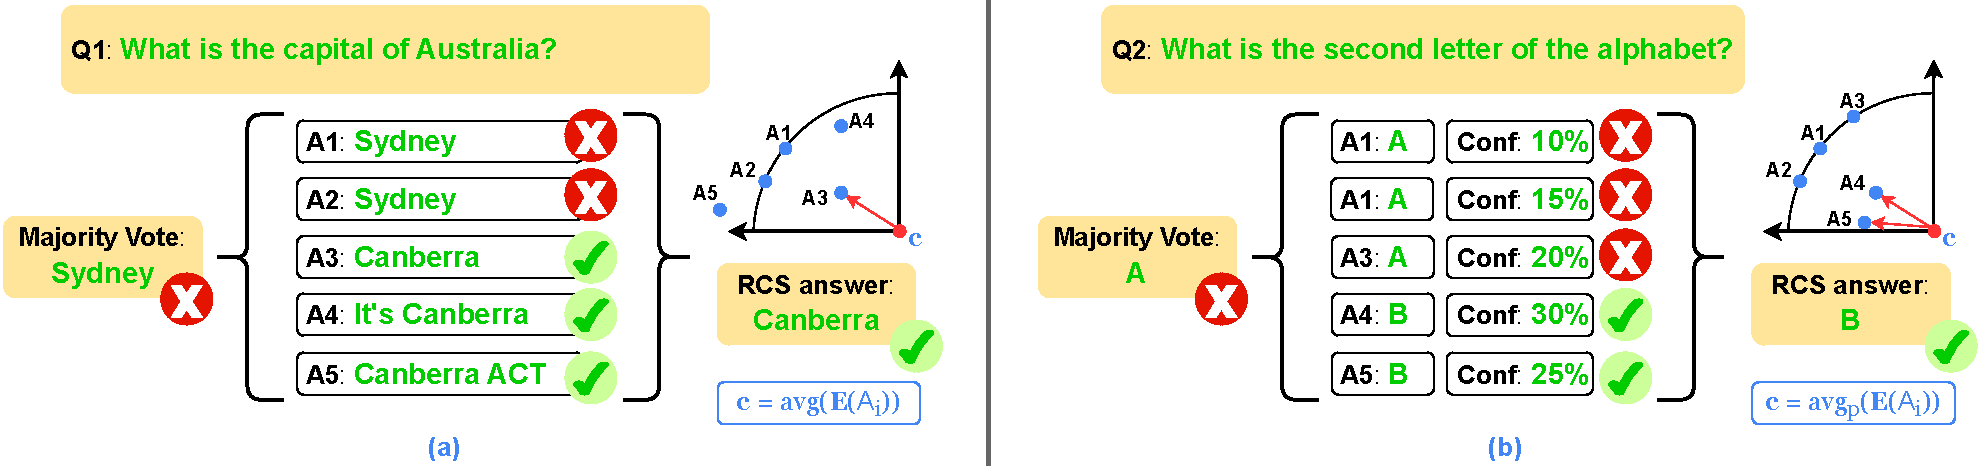
\includegraphics[width=\textwidth]{plots/RDS_overview.pdf}
    \caption{
        RCS overview and representative failure modes of majority voting.
        (a) Majority voting ignores semantically similar answers by treating surface forms independently.
        (b) It also fails to select high-confidence but minority answers.
        RCS addresses both issues by mapping answers into an embedding space via Encoder $\mathbf{E}$ and estimating a centroid $\mathbf{c}$, either \textit{uniformly} or \textit{probability-weighted} over answer embeddings. Additional qualitative examples are provided in Section~\ref{sec:qualitative}.}
    \label{fig:overview}
\end{figure*}